\documentclass[11pt,a4paper]{article}

\usepackage[utf8]{inputenc}
\usepackage[T1]{fontenc}
\usepackage{lmodern}
\usepackage[margin=2.5cm]{geometry}
\usepackage{graphicx}
\usepackage{booktabs}
\usepackage{amsmath}
\usepackage{amssymb}
\usepackage{hyperref}
\usepackage{caption}
\usepackage{float}
\usepackage{array}
\usepackage{setspace}

\hypersetup{
    colorlinks=true,
    linkcolor=black,
    citecolor=blue,
    urlcolor=blue
}

\begin{document}

%%============================================================
%% COVER PAGE
%%============================================================
\begin{titlepage}
\centering
\vspace*{1.5cm}
{\large\textbf{The Faculty of Engineering}\\[0.3cm]
\textbf{The Maersk Mc-Kinney Moller Institute}\\[0.3cm]
\textbf{Project Report}}

\vspace{1.5cm}

\begin{tabular}{|p{7.5cm}|p{7.5cm}|}
\hline
\textbf{Student Name:} & \textbf{Student ID Number:} \\[0.4cm]
Amirhossein Taleshinosrati & 4144308 \\[0.3cm]
\hline
\end{tabular}

\vspace{0.8cm}

\begin{tabular}{|p{4.2cm}|p{10.8cm}|}
\hline
Class and Year         & Master of Science in Engineering Drone Technology and Autonomous Systems 2025--2027 \\
\hline
Subject Code and Name  & T550021101-1-F25 Tools of Artificial Intelligence (F25) \\
\hline
Lecturer Name(s)       & Vinay Chakravarthi Gogineni / Smith Khare / Orkun Furat \\
\hline
Title                  & EMG-Based Hand Gesture Classification Using Machine Learning: A Comparative Study of Feature Sets and Classifiers \\
\hline
Other Group Members    & (working alone) \\
\hline
Submission Date        & 24-05-2026 \\
\hline
\end{tabular}

\vspace{1.5cm}

\begin{flushleft}
\textbf{Academic Integrity and Plagiarism}

\vspace{0.3cm}
{\small Plagiarism is the act of copying, including or directly quoting from, the work of another without
adequate acknowledgment. All work submitted by students for assessment purposes is accepted on the
understanding that it is their own work and written in their own words except where explicitly referenced
using the correct format. For example, you must NOT copy information, ideas, portions of text, data,
figures, computer programs, etc.\ from anywhere without giving a reference to the source. Sources can
include websites, other students' work, books, journal articles, reports, etc. Self-plagiarism or
auto-plagiarism is where a student re-uses work previously submitted to another course within the SDU
or other Universities.

\vspace{0.3cm}
You must ensure that you have read the SDU regulations relating to plagiarism.}

\vspace{0.8cm}
{\normalsize\textit{I have read and understood the SDU code of practice on plagiarism and confirm that
the content of this document is my own work and has not been plagiarized.}}

\vspace{1.2cm}
Student's signature \hspace{1.5cm} \framebox[8cm]{\rule{0pt}{2cm}}
\end{flushleft}
\end{titlepage}

%%============================================================
%% ABSTRACT  (page 1)
%%============================================================
\setcounter{page}{1}
\begin{abstract}
This study presents a machine learning pipeline for binary classification of the hand gestures Rock and Paper from single-channel Electromyography (EMG) signals recorded at 256~Hz. The dataset contains 5\,850 trials (2\,909 Rock, 2\,941 Paper), each with 1\,024 time-series samples ($\approx$4~s). Twenty-six features were extracted per trial across four domains: statistical (8), time-domain (7), frequency-domain (6), and entropy (5). Feature selection combined the Kruskal-Wallis non-parametric test ($p < 0.05$) with Principal Component Analysis (PCA) retaining 95\% of the explained variance. Three classifiers were evaluated: Random Forest (RF), Support Vector Machine with RBF kernel (SVM-RBF), and eXtreme Gradient Boosting (XGBoost), under three validation strategies: hold-out (80/20 split), 5-fold stratified cross-validation, and GridSearchCV hyperparameter tuning. Among the evaluated models, SVM-RBF gave the best overall results on this dataset, with an F1 score of 80.63\% and an AUC of 0.875. A feature-domain ablation study showed that combining all feature types (79.49\%) outperformed any individual domain, with entropy features being the strongest single group (75.04\%) and frequency-domain features the weakest (68.97\%). These results fall within the range reported in the literature for single-channel binary EMG gesture classification and suggest that multi-domain feature fusion is useful when paired with a kernel-based classifier.
\end{abstract}

\newpage

%%============================================================
%% TABLE OF CONTENTS
%%============================================================
\tableofcontents
\newpage

%%============================================================
%% MAIN BODY
%%============================================================

\section{Introduction}

Gesture recognition is a core problem in human-computer interaction (HCI), enabling control of machines through hand movements. Applications include prosthetic limb control, rehabilitation robotics, sign language interpretation, and industrial automation~\cite{phinyomark2012feature}. Electromyography (EMG) is one of the most widely used sensing modalities because it directly measures the electrical activity of skeletal muscles during voluntary movement.

EMG-based classification is challenging due to signal noise, subject dependence, and non-stationarity. Despite the popularity of deep learning, classical pipelines combining handcrafted features with supervised classifiers remain competitive on moderate-sized datasets because they are interpretable and computationally efficient~\cite{atzori2016deep}. This project implements and evaluates such a pipeline for distinguishing Rock and Paper gestures from single-channel EMG signals, covering feature extraction, statistical feature selection, PCA dimensionality reduction, comparison of three classifiers under three validation strategies, and a feature-domain ablation study.

\section{Related Works}

Phinyomark et al.~\cite{phinyomark2012feature} evaluated time-domain EMG features and found that RMS and Zero Crossing Rate are among the most discriminative features for gesture recognition, with binary classification accuracies of 70--85\%, providing a reference point for the present results.

Oskoei and Hu~\cite{oskoei2007myoelectric} benchmarked several classifiers on upper-limb EMG data and found SVM with an RBF kernel outperformed k-NN and LDA, especially for non-linear class boundaries. Their reported SVM accuracies of 80--95\% used multi-channel (6--10 channel) recordings, which explains the expected performance gap relative to the single-channel setup used here.

Atzori et al.~\cite{atzori2016deep} evaluated Random Forest on the NinaPro EMG database and found it competitive with deep learning while remaining interpretable. XGBoost~\cite{chen2016xgboost} is a regularised gradient-boosted ensemble that has performed well across many benchmarks. Including RF and XGBoost alongside SVM-RBF allows a comparison of tree-based and kernel-based approaches. The Kruskal-Wallis test has been used for feature selection in biomedical signals without assuming normality~\cite{subasi2013classification}, which is important for entropy-based features.

\section{Methodology}

\subsection{Dataset Description}

The dataset was provided by the Maersk Mc-Kinney Moller Institute at the University of Southern Denmark as part of the Tools of Artificial Intelligence course. It contains single-channel EMG recordings for three hand gestures (Rock, Paper, Scissor) stored as separate CSV files. For this binary classification task, \texttt{RockData.csv} (2\,909 trials, label = 0) and \texttt{PaperData.csv} (2\,941 trials, label = 1) were merged into a combined dataset of 5\,850 trials. Each trial contains 1\,024 time-series samples recorded at a sampling frequency of $f_s = 256$~Hz, which corresponds to roughly 4 seconds of signal per trial. The class distribution is close to balanced (49.7\% Rock, 50.3\% Paper), so no class balancing was applied. Figure~\ref{fig:eda} shows the exploratory visualisation of the dataset.

\begin{figure}[H]
\centering
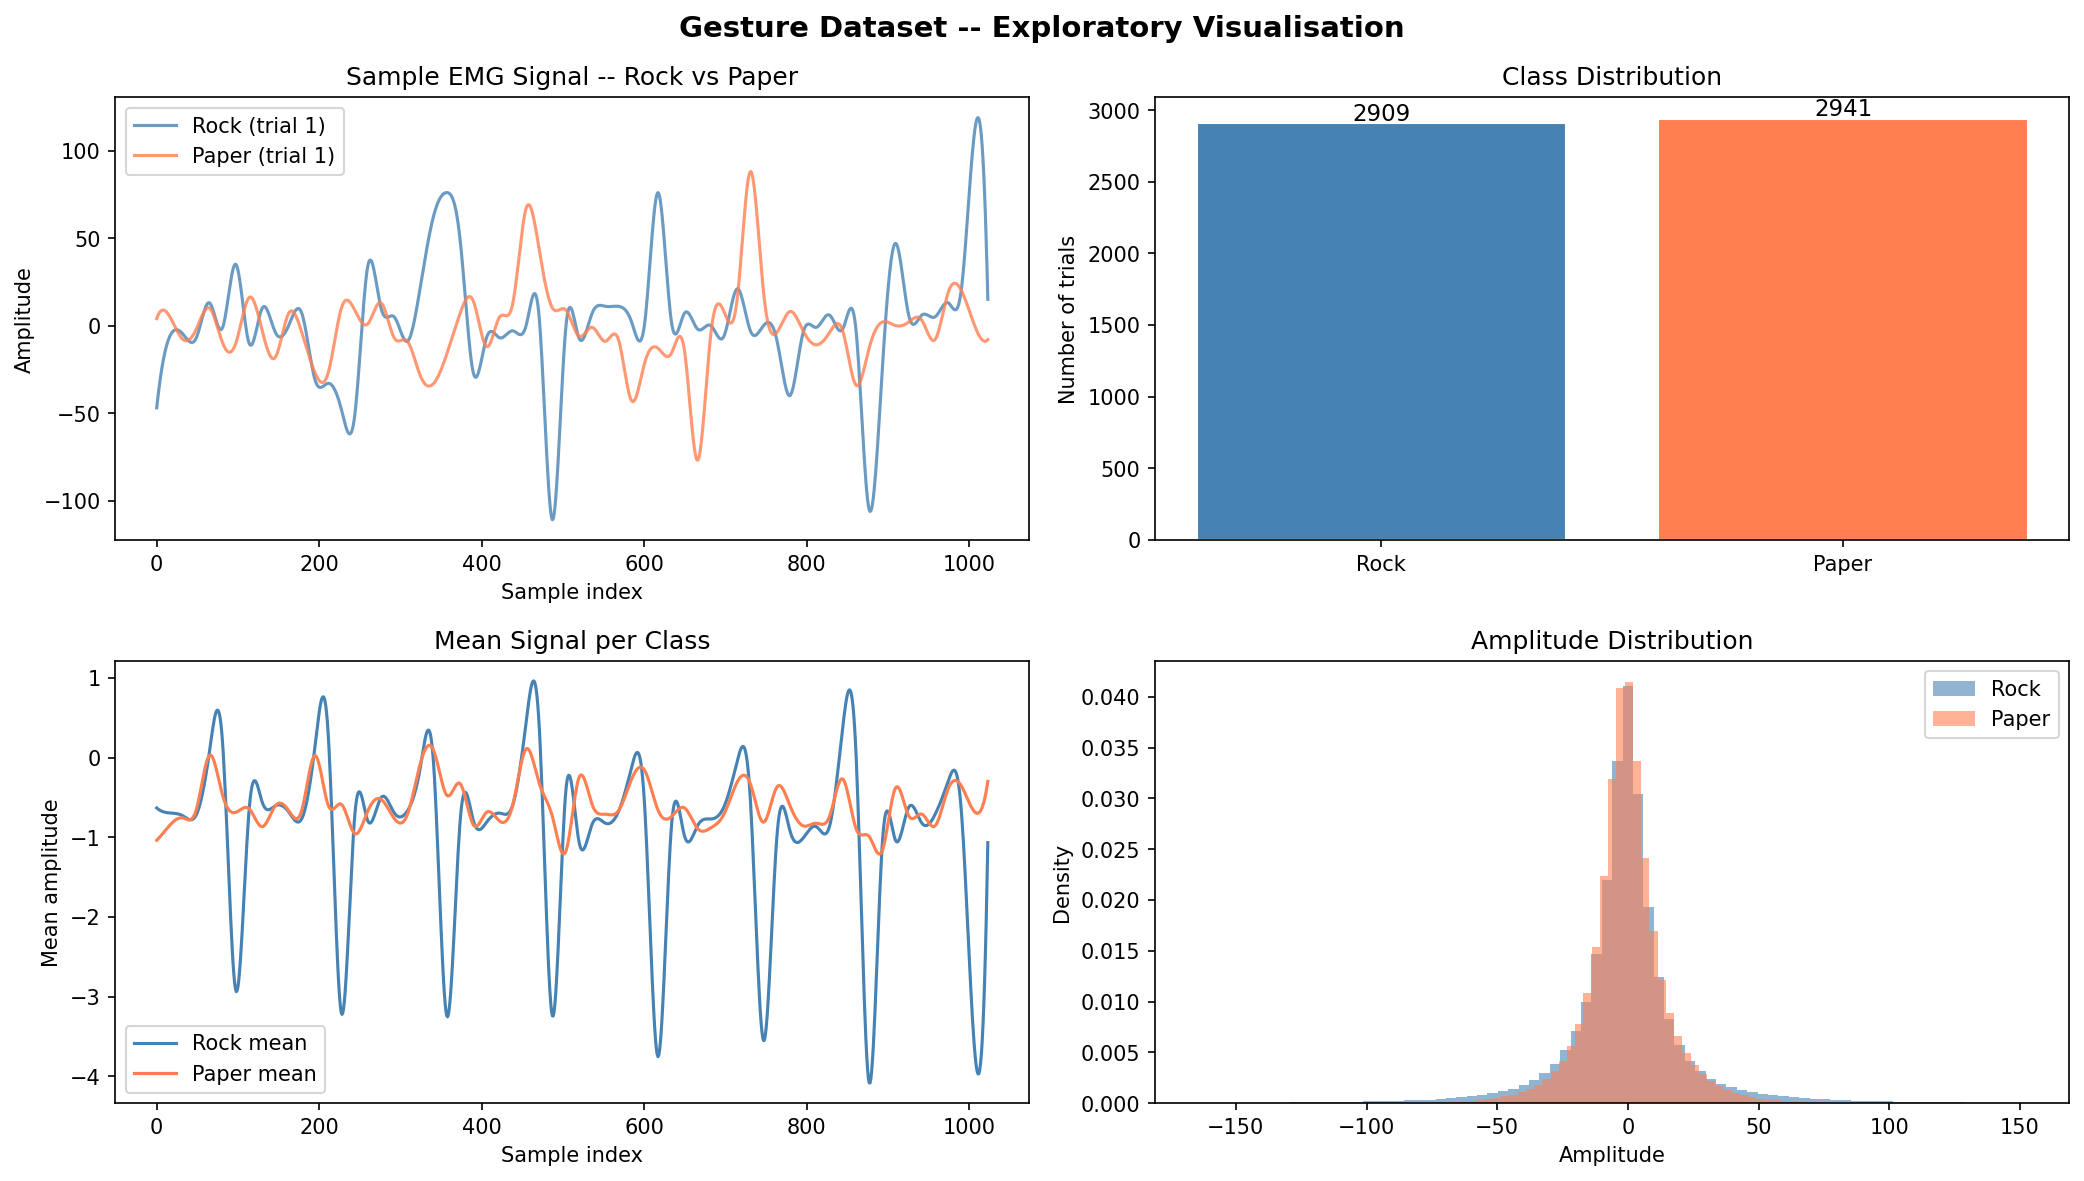
\includegraphics[width=0.78\textwidth]{figures/eda.png}
\caption{Exploratory dataset visualisation: (top-left) sample EMG signals; (top-right) class distribution; (bottom-left) mean signal per class; (bottom-right) amplitude density distributions showing substantial overlap due to single-channel limitations.}
\label{fig:eda}
\end{figure}

\subsection{Data Preprocessing}

\textbf{Missing values.} The feature matrix ($5\,850 \times 1\,024$) contained zero NaN values, so no imputation was needed~\cite{little2002statistical}. \textbf{Signal filtering.} Signals were already filtered prior to recording; no additional filtering was applied. \textbf{Data leakage prevention.} \texttt{StandardScaler} and PCA were fit exclusively on training data and applied to the test fold, ensuring no test-set information leaked into feature transformation.

\subsection{Feature Extraction}

Twenty-six features were extracted from each trial across four domains. Using more than one feature domain is motivated by the complementary nature of different feature types: statistical features capture the amplitude distribution, time-domain features capture temporal dynamics, frequency-domain features capture spectral content, and entropy features capture signal complexity. All features were computed on the full 1\,024-sample trial signal.

\begin{itemize}
    \item \textbf{Statistical features (8):} Mean, Median, Standard Deviation, Variance, Skewness, Kurtosis, Range, Interquartile Range (IQR).
    \item \textbf{Time-domain features (7):} Root Mean Square (RMS), Zero Crossing Rate (ZCR), Autocorrelation, Mean Absolute Deviation (MAD), Maximum, Minimum, Signal Energy.
    \item \textbf{Frequency-domain features (6):} Dominant Frequency, Total Power, Band Power (0.5--40~Hz), Mean Frequency, Median Frequency, and Frequency Variance, computed using Welch's Power Spectral Density estimate at $f_s = 256$~Hz.
    \item \textbf{Entropy features (5):} Sample Entropy, Spectral Entropy, Permutation Entropy, SVD Entropy, and Lempel-Ziv (LZiv) Complexity, which quantify signal regularity and complexity.
\end{itemize}

Key feature definitions are given below. The mean and standard deviation describe the signal amplitude distribution:
\begin{equation}
\mu = \frac{1}{N} \sum_{i=1}^{N} x_i
\end{equation}
\begin{equation}
\sigma = \sqrt{\frac{1}{N} \sum_{i=1}^{N} (x_i - \mu)^2}
\end{equation}
where $x_i$ is the $i$-th sample and $N = 1\,024$ is the number of samples per trial. RMS and Signal Energy describe signal power:
\begin{equation}
\text{RMS} = \sqrt{\frac{1}{N} \sum_{i=1}^{N} x_i^2}
\end{equation}
\begin{equation}
E = \sum_{i=1}^{N} x_i^2
\end{equation}

\subsection{Feature Selection}

\textbf{Step 1 --- Standardisation.} All 26 features were standardised to zero mean and unit variance using \texttt{StandardScaler} before feature selection, since both the Kruskal-Wallis test and PCA are sensitive to differences in feature scale. As noted above, the scaler was fit on training data only.

\textbf{Step 2 --- Kruskal-Wallis test.} The non-parametric Kruskal-Wallis H-test was applied to each feature to check whether its distribution differed significantly between Rock and Paper classes. Features with $p < 0.05$ were retained. The Kruskal-Wallis test was chosen over ANOVA because it does not assume normality, which is an important consideration for entropy-based measures. Figure~\ref{fig:boxplot} shows the four most discriminative features.

\begin{figure}[H]
\centering
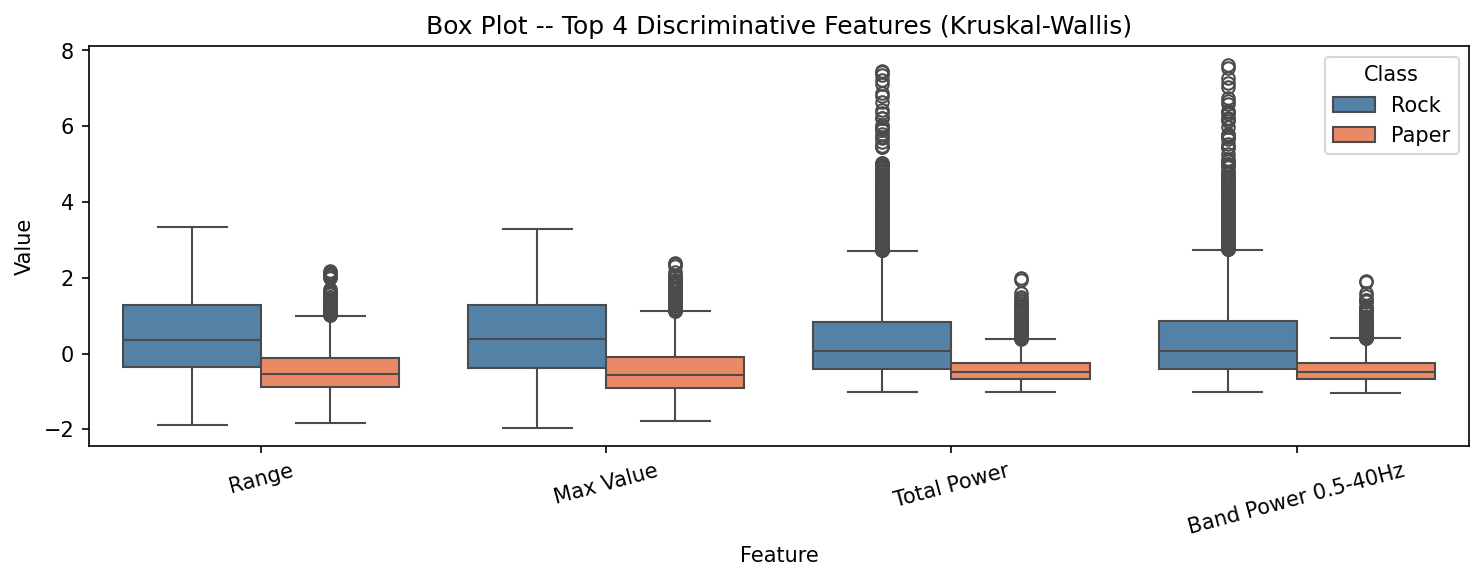
\includegraphics[width=0.75\textwidth]{figures/boxplot.png}
\caption{Box plots of the four most discriminative features (Kruskal-Wallis, $p < 0.05$). Rock (blue) shows consistently higher median values than Paper (orange).}
\label{fig:boxplot}
\end{figure}

\textbf{Step 3 --- PCA.} PCA was applied to the selected features, retaining components that cumulatively explain 95\% of variance, removing redundant information and reducing overfitting risk. Figure~\ref{fig:pca} shows the 2D projection.

\begin{figure}[H]
\centering
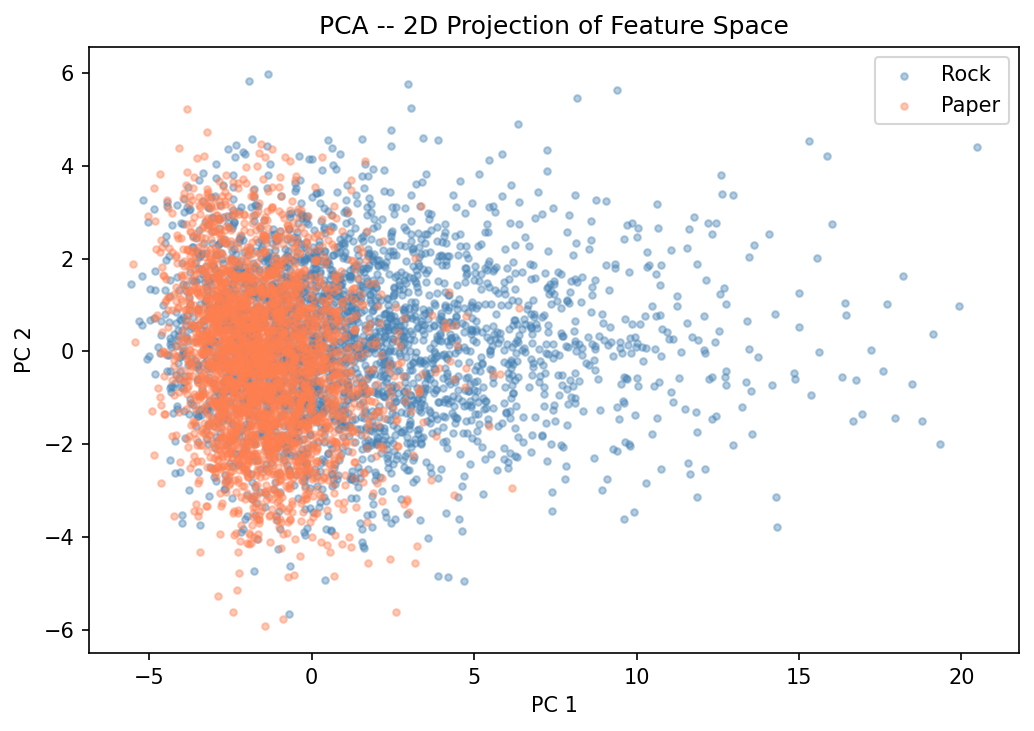
\includegraphics[width=0.55\textwidth]{figures/pca.png}
\caption{2D PCA projection after Kruskal-Wallis selection. Partial separation along PC~1 is visible; overlap reflects single-channel limitations.}
\label{fig:pca}
\end{figure}

\subsection{Classification Models}

Three classifiers from different algorithmic families were implemented and compared:
\begin{itemize}
    \item \textbf{Random Forest (RF):} An ensemble of 100 decision trees trained on bootstrap samples. Each tree votes independently and the majority decides the prediction. RF is fairly robust to overfitting and handles non-linear boundaries well~\cite{breiman2001random}.
    \item \textbf{SVM with RBF kernel (SVM-RBF):} Maps the feature space to a higher-dimensional space using the kernel $K(x_i, x_j) = \exp\left(-\|x_i - x_j\|^2 / 2\sigma^2\right)$, which allows non-linear classification while maximising the margin between classes~\cite{oskoei2007myoelectric}.
    \item \textbf{XGBoost:} A regularised gradient-boosted tree ensemble that iteratively fits trees to the residual errors of previous trees, with L1 and L2 regularisation to control overfitting~\cite{chen2016xgboost}.
\end{itemize}

\subsection{Validation Strategies}

\begin{itemize}
    \item \textbf{Hold-out (80/20 split):} 4\,680 training samples and 1\,170 test samples, using stratified random sampling to preserve class proportions. This is fast and simple, but the result depends on the particular split chosen.
    \item \textbf{5-Fold Stratified Cross-Validation:} The dataset was partitioned into 5 folds of roughly equal size. Each fold served once as the test set while the remaining 4 folds were used for training, and results were averaged across folds. As noted above, the scaler and PCA were re-fit inside each training fold.
    \item \textbf{GridSearchCV:} Exhaustive hyperparameter search applied to all three classifiers using 5-fold CV: RF over \texttt{n\_estimators}, \texttt{max\_depth}, \texttt{min\_samples\_split} (18 configs, 90 fits); SVM-RBF over $C$ and $\gamma$ (12 configs, 60 fits); XGBoost over \texttt{n\_estimators}, \texttt{max\_depth}, \texttt{learning\_rate} (18 configs, 90 fits).
\end{itemize}

All experiments were implemented in Python using Scikit-learn and XGBoost. A fixed \texttt{random\_state} of 42 was used where applicable so the train-test split and model training are reproducible.

\section{Results}

\subsection{Feature Set Comparison}

To quantify the contribution of each feature domain, a Random Forest was trained and evaluated under hold-out validation for each feature group separately and for the combined 26-feature set. Results are shown in Table~\ref{tab:featureset} and Figure~\ref{fig:featureset}.

\begin{table}[H]
\centering
\caption{Classification accuracy by feature domain using Random Forest (100 trees, hold-out 80/20). Best result in bold.}
\label{tab:featureset}
\begin{tabular}{lc}
\toprule
\textbf{Feature Set} & \textbf{Hold-out Accuracy (\%)} \\
\midrule
Statistical only (8 features) & 73.08 \\
Time-domain only (7 features) & 73.33 \\
Frequency-domain only (6 features) & 68.97 \\
Entropy only (5 features) & 75.04 \\
\textbf{All features combined (26 features)} & \textbf{79.49} \\
\bottomrule
\end{tabular}
\end{table}

\begin{figure}[H]
\centering
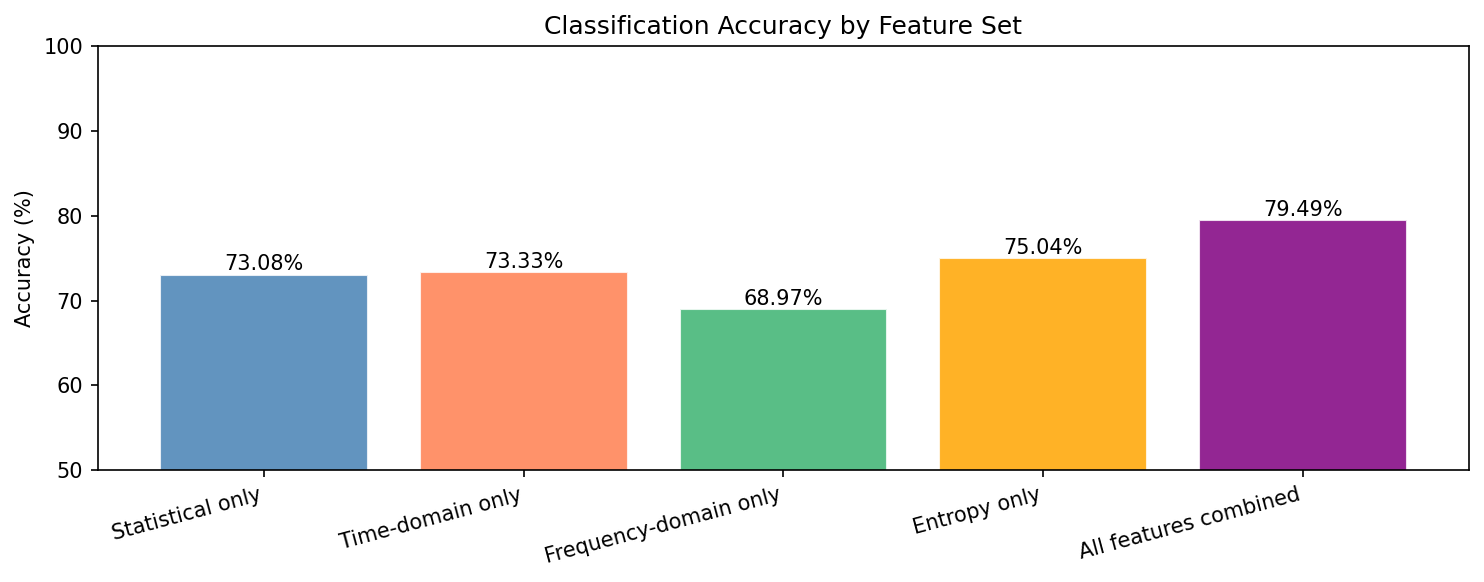
\includegraphics[width=0.72\textwidth]{figures/featureset.png}
\caption{Accuracy by feature domain. All-features combined (79.49\%) outperforms any individual domain. Entropy is strongest single group (75.04\%); frequency-domain is weakest (68.97\%).}
\label{fig:featureset}
\end{figure}

Combining all feature types gave a 4.45 percentage point gain over the best single domain (entropy, 75.04\%), confirming complementary information across domains. Frequency-domain features were weakest (68.97\%), consistent with both gestures involving static postures with limited spectral differences.

\subsection{Feature Importance}

To identify which individual features drive classification, a separate Random Forest (100 trees) was fitted on the Kruskal-Wallis selected features before PCA reduction, so that importances map back to interpretable feature names. Results are shown in Figure~\ref{fig:importance}.

\begin{figure}[H]
\centering
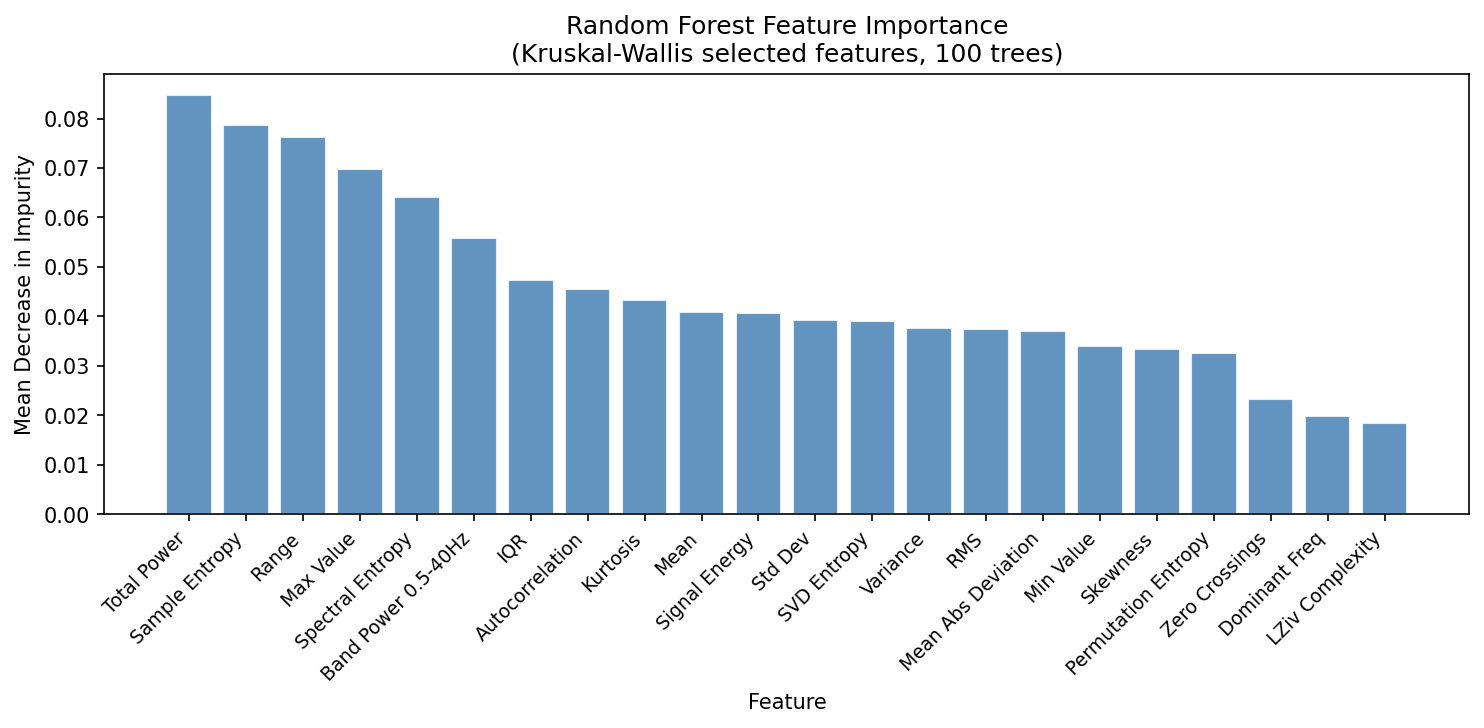
\includegraphics[width=0.78\textwidth]{figures/importance.png}
\caption{Random Forest feature importance (mean decrease in impurity) for Kruskal-Wallis selected features. Higher values indicate greater discriminative power for Rock vs.\ Paper.}
\label{fig:importance}
\end{figure}

\subsection{Classifier Performance}

Table~\ref{tab:classifier} reports the performance metrics for all three classifiers, evaluated on the combined 26-feature set after Kruskal-Wallis selection and PCA reduction (95\% variance retained). Figure~\ref{fig:cmroc} shows the corresponding confusion matrices and ROC curves.

\begin{table}[H]
\centering
\caption{Performance metrics for all classifiers under hold-out validation (80/20 split). Best per-metric values in bold.}
\label{tab:classifier}
\begin{tabular}{lccccc}
\toprule
\textbf{Classifier} & \textbf{Accuracy} & \textbf{Sensitivity} & \textbf{Specificity} & \textbf{F1 Score} & \textbf{AUC} \\
\midrule
Random Forest & 78.38\% & 79.42\% & 77.32\% & 78.69\% & 0.866 \\
\textbf{SVM (RBF)} & \textbf{78.97\%} & \textbf{87.07\%} & 70.79\% & \textbf{80.63\%} & \textbf{0.875} \\
XGBoost & 75.90\% & 77.55\% & 74.23\% & 76.38\% & 0.850 \\
\bottomrule
\end{tabular}
\end{table}

\begin{figure}[H]
\centering
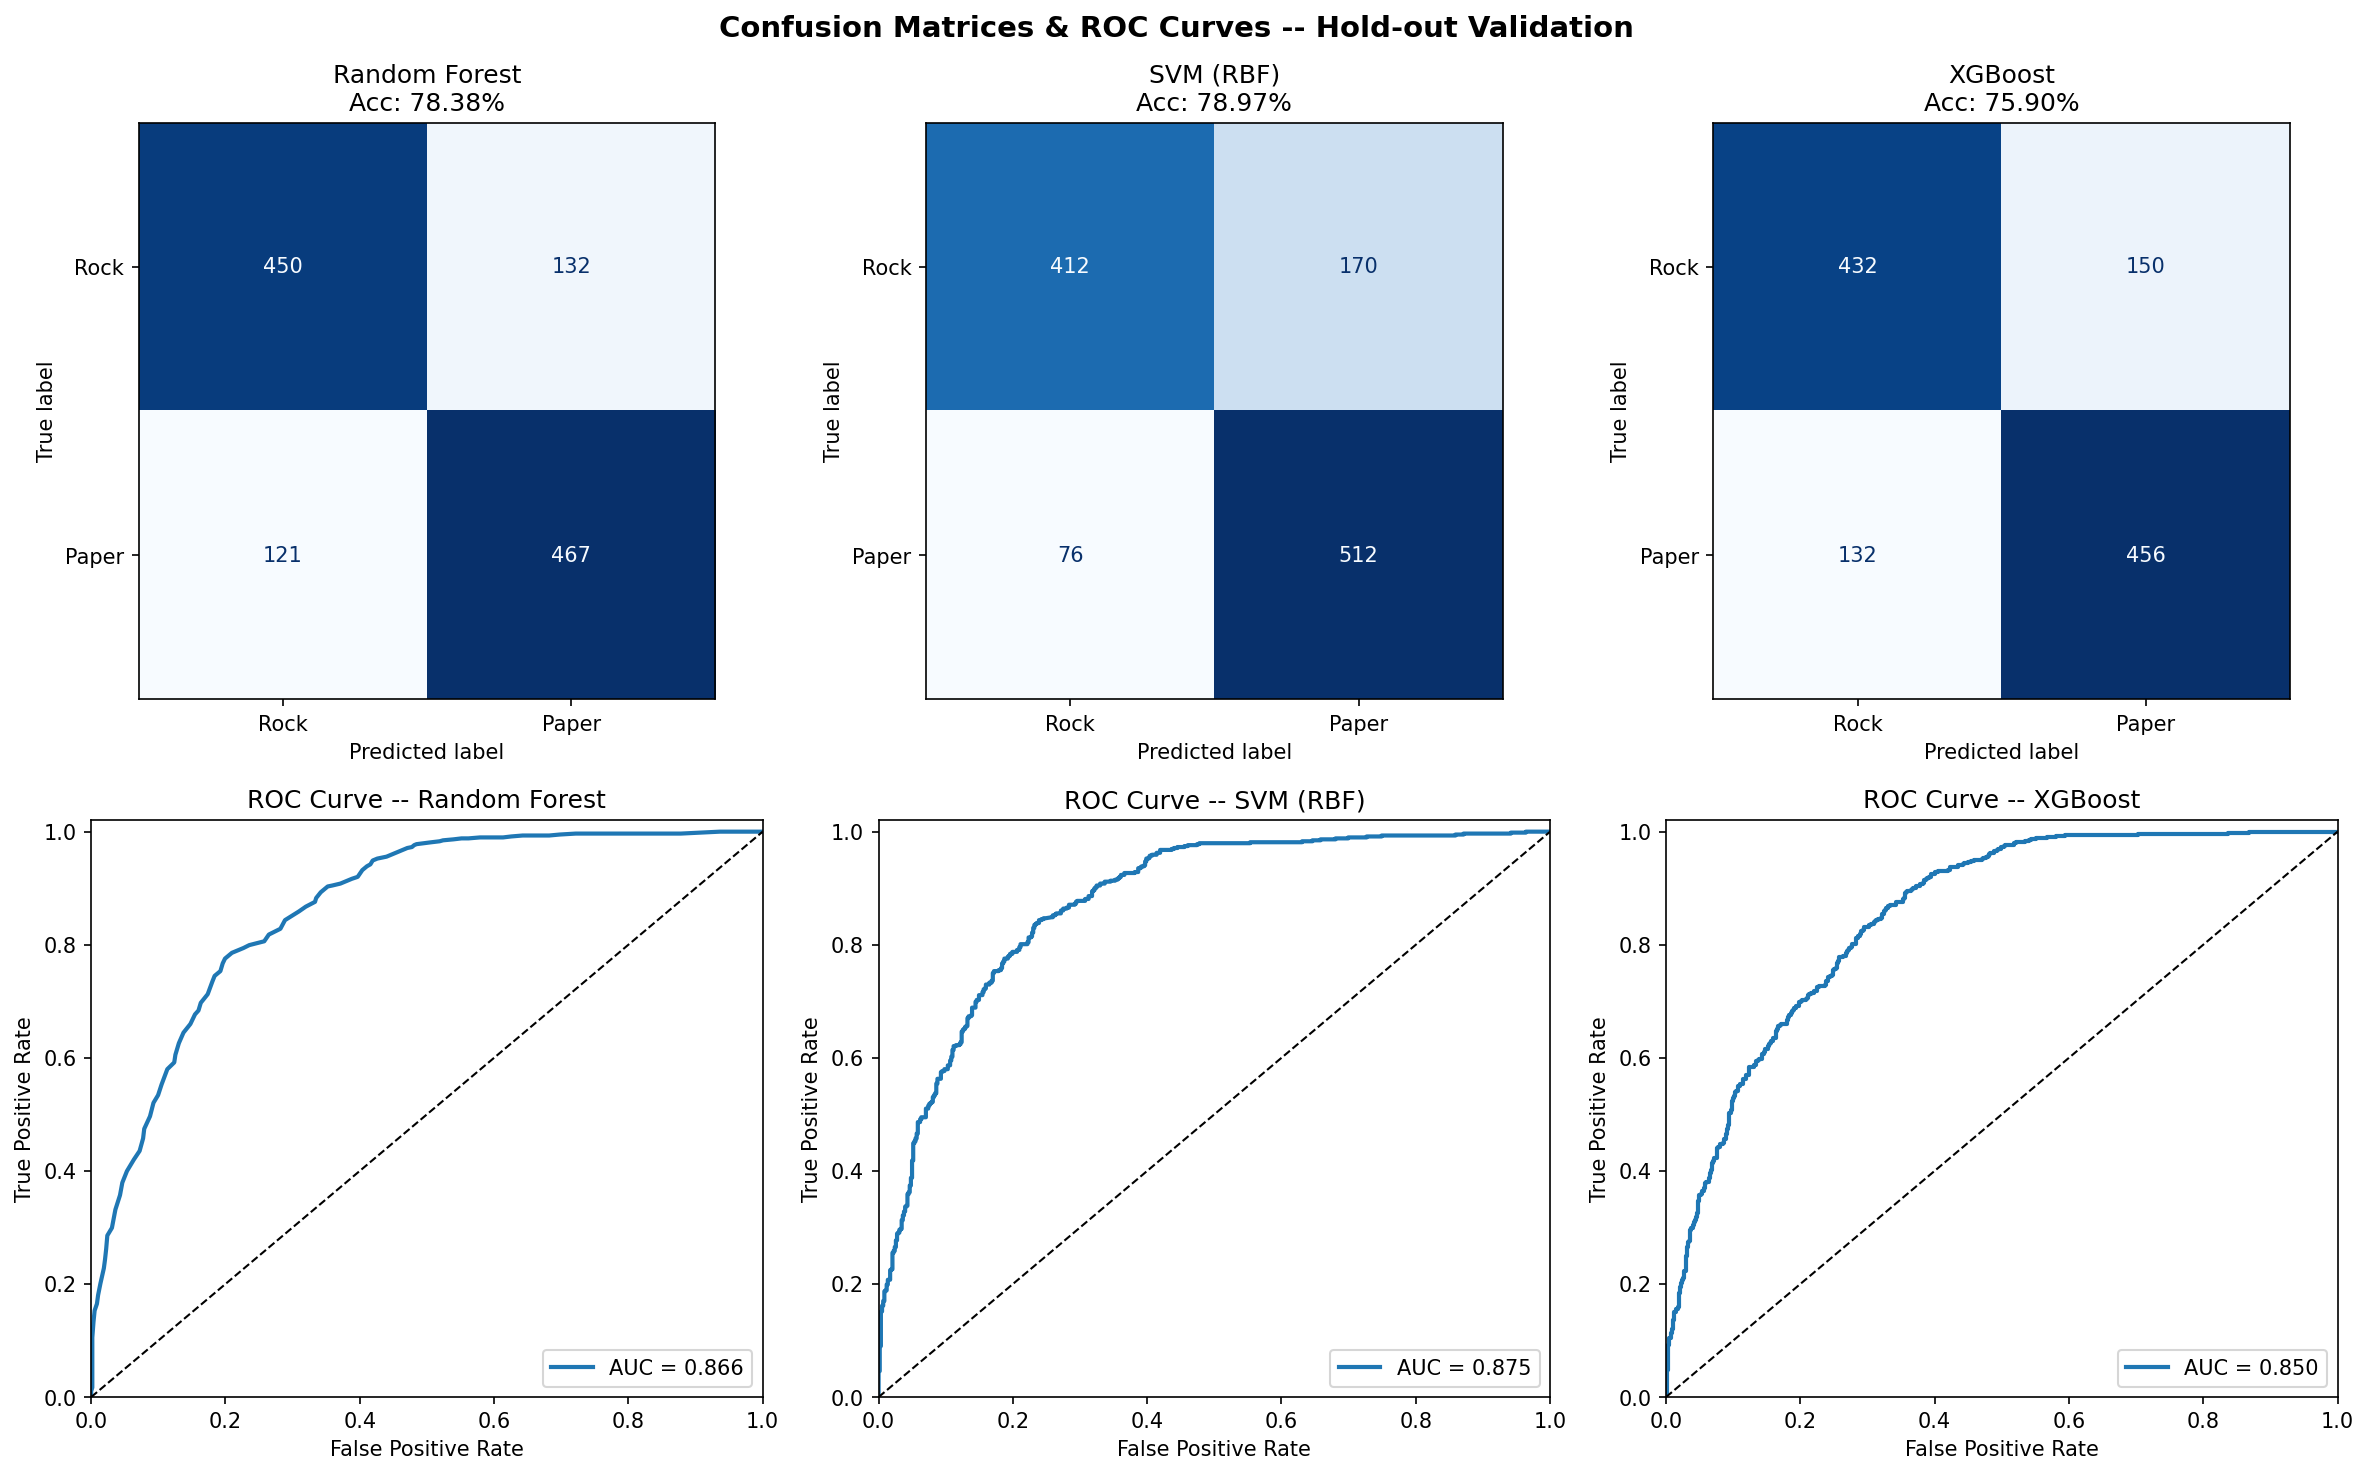
\includegraphics[width=0.92\textwidth]{figures/cmroc.png}
\caption{Confusion matrices and ROC curves for all three classifiers under hold-out validation.}
\label{fig:cmroc}
\end{figure}

SVM-RBF achieved the highest accuracy (78.97\%), F1 (80.63\%), and AUC (0.875). Its high sensitivity (87.07\%) comes at the cost of lower specificity (70.79\%), whereas Random Forest showed a more balanced trade-off (sensitivity 79.42\%, specificity 77.32\%). XGBoost was weakest across all metrics (accuracy 75.90\%, AUC 0.850).

\subsection{Validation Strategy Comparison}

Table~\ref{tab:validation} and Figures~\ref{fig:cvbox}--\ref{fig:valcompare} compare the three validation strategies across all classifiers.

\begin{table}[H]
\centering
\caption{Validation strategy comparison. GridSearchCV applied to all three classifiers using 5-fold CV (RF: 18 configs, best CV 77.09\%; SVM: 12 configs, best CV 77.86\%; XGBoost: 18 configs, best CV 76.92\%).}
\label{tab:validation}
\begin{tabular}{lccc}
\toprule
\textbf{Classifier} & \textbf{Hold-out (\%)} & \textbf{CV Mean $\pm$ Std (\%)} & \textbf{GridSearch (\%)} \\
\midrule
Random Forest & 78.38 & $76.99 \pm 0.79$ & 78.38 \\
\textbf{SVM (RBF)} & \textbf{78.97} & $\mathbf{77.76 \pm 0.83}$ & \textbf{79.40} \\
XGBoost & 75.90 & $75.52 \pm 0.87$ & 78.12 \\
\bottomrule
\end{tabular}
\end{table}

\begin{figure}[H]
\centering
\begin{minipage}{0.48\textwidth}
    \centering
    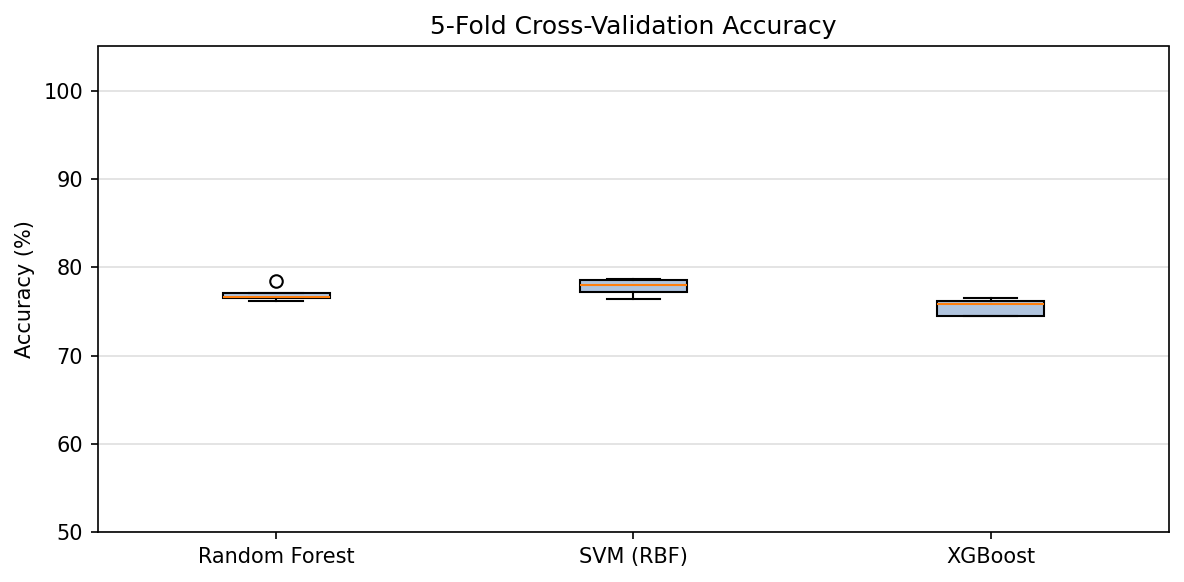
\includegraphics[width=\textwidth]{figures/cvbox.png}
    \caption{5-fold CV accuracy distributions. SVM (RBF) had the highest mean (77.76\% $\pm$ 0.83\%).}
    \label{fig:cvbox}
\end{minipage}\hfill
\begin{minipage}{0.48\textwidth}
    \centering
    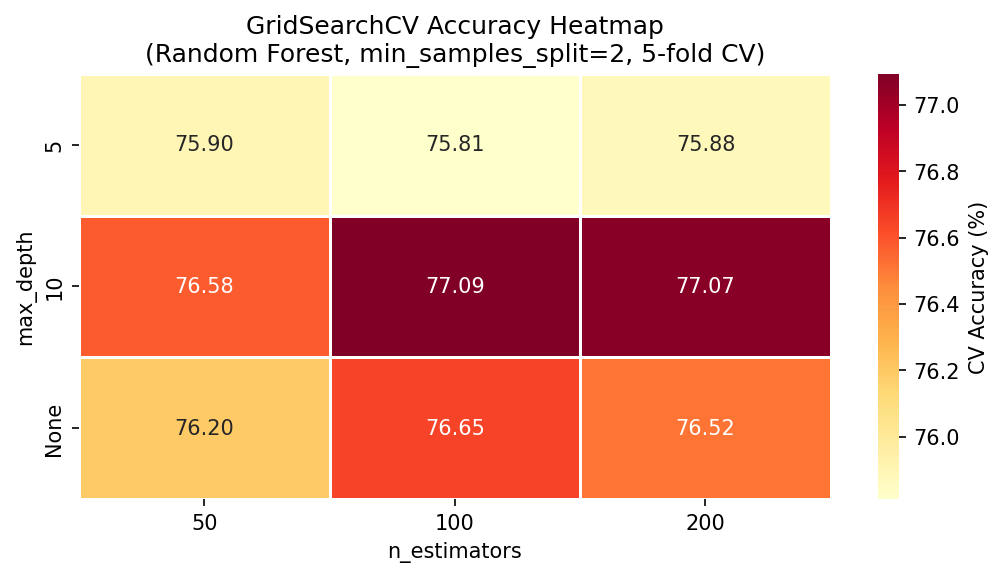
\includegraphics[width=\textwidth]{figures/gridheatmap.png}
    \caption{GridSearchCV heatmap for RF (5-fold CV). Optimal: \texttt{n\_estimators=100}, \texttt{max\_depth=10}; best CV 77.09\%.}
    \label{fig:gridheatmap}
\end{minipage}
\end{figure}

\begin{figure}[H]
\centering
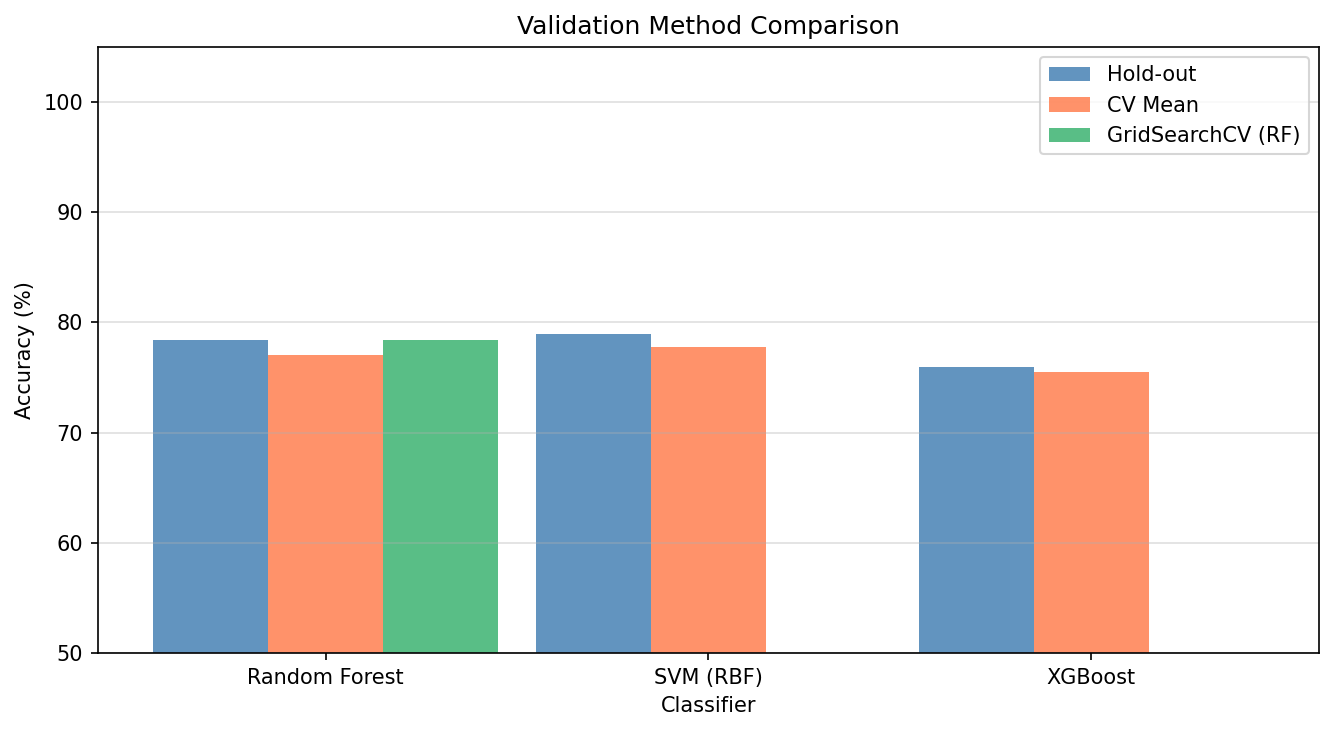
\includegraphics[width=0.78\textwidth]{figures/valcompare.png}
\caption{Grouped bar chart comparing hold-out, CV mean, and GridSearchCV accuracy for all three classifiers.}
\label{fig:valcompare}
\end{figure}

SVM-RBF led across all strategies: hold-out (78.97\%), CV (77.76\% $\pm$ 0.83\%), and GridSearch (79.40\%). The small hold-out vs.\ CV gap is typical of single-split evaluation. GridSearch confirmed near-optimal defaults: RF (\texttt{n\_estimators=100}, \texttt{max\_depth=10}, 78.38\%), SVM-RBF ($C=10$, $\gamma=0.01$, 79.40\%), XGBoost (\texttt{n\_estimators=100}, \texttt{max\_depth=3}, \texttt{learning\_rate=0.1}, 78.12\%).

\section{Discussion and Conclusions}

The primary finding is that SVM-RBF is the most effective classifier, achieving the highest hold-out accuracy (78.97\%), F1 score (80.63\%), and AUC (0.875), consistent with the literature~\cite{oskoei2007myoelectric}. Its high sensitivity (87.07\%) reflects a tendency to classify borderline trials as Paper, trading lower specificity (70.79\%) for fewer missed Paper gestures.

The ablation study confirmed that no single feature domain suffices alone, and multi-domain fusion is essential. Entropy features were most informative (75.04\%) since signal complexity differs between Rock and Paper activation patterns, while frequency features performed weakest (68.97\%) due to both gestures involving static muscle postures with limited spectral differences.

\textbf{Benchmarks.} The 78.97\% accuracy is within the 70--85\% range reported by Phinyomark et al.~\cite{phinyomark2012feature} for single-channel binary tasks, and below the 80--95\% of Oskoei and Hu~\cite{oskoei2007myoelectric} who used 6--10 channels, confirming that single-channel measurement is the primary limiting factor.

\textbf{Limitations and future work.} The 75--79\% accuracy range reflects the inherent difficulty of single-channel EMG classification. Multi-channel recording, subject-independent cross-validation (LOSO), and deep learning architectures (1D CNNs, BiLSTMs) are natural extensions to improve performance.

\section{Reflection}

This project gave me hands-on experience with the full machine learning pipeline applied to physiological signal data. The most technically demanding part was implementing the entropy features, particularly Sample Entropy and LZiv Complexity, which required explicit float64 conversion and binary signal thresholding to remain numerically stable across all 5\,850 trials. Debugging the Kruskal-Wallis \texttt{ValueError} caused by zero-variance features after standardisation was resolved by wrapping the test in a try-except block.

The feature-domain ablation experiment was a particularly valuable addition, turning a broad task requirement into a concrete result: entropy features were the most informative single domain, while frequency-domain features contributed least. The data leakage prevention step — fitting the scaler and PCA only on training folds — reinforced the importance of correct cross-validation implementation.

Working individually pushed me to be more systematic about comparison, covering multiple classifiers, validation strategies, and feature sets in a structured way. Overall, the project strengthened my understanding of preprocessing decisions, feature engineering, hyperparameter tuning, and result interpretation through confusion matrices, ROC curves, and feature importance rankings.

\begin{thebibliography}{9}

\bibitem{atzori2016deep}
Atzori, M., Cognolato, M., and M\"{u}ller, H. (2016).
Deep learning with convolutional neural networks applied to electromyography data: A resource for the classification of movements for prosthetic hands.
\emph{Frontiers in Neurorobotics}, 10:9.

\bibitem{breiman2001random}
Breiman, L. (2001).
Random forests.
\emph{Machine Learning}, 45(1):5--32.

\bibitem{chen2016xgboost}
Chen, T. and Guestrin, C. (2016).
XGBoost: A scalable tree boosting system.
In \emph{Proceedings of the 22nd ACM SIGKDD International Conference on Knowledge Discovery and Data Mining}, pages 785--794.

\bibitem{little2002statistical}
Little, R. J. A. and Rubin, D. B. (2002).
\emph{Statistical Analysis with Missing Data}.
Wiley-Interscience, 2nd edition.

\bibitem{oskoei2007myoelectric}
Oskoei, M. A. and Hu, H. (2007).
Myoelectric control systems --- A survey.
\emph{Biomedical Signal Processing and Control}, 2(4):275--294.

\bibitem{phinyomark2012feature}
Phinyomark, A., Phukpattaranont, P., and Limsakul, C. (2012).
Feature reduction and selection for EMG signal classification.
\emph{Expert Systems with Applications}, 39(8):7420--7431.

\bibitem{subasi2013classification}
Subasi, A. (2013).
Classification of EMG signals using PSO optimized SVM for diagnosis of neuromuscular disorders.
\emph{Computers in Biology and Medicine}, 43(5):576--586.

\end{thebibliography}

\end{document}
